\section{Superconductivity}
\subsection{Phenomenology and Historical Background}
We will not provide a large background of the phenomenology of superconductivity - the first 2-3 pages of any textbook section about it will explain it in depth. We just give a couple points and then explain the Cooper problem which is the microscopic foundations for the effect.

\begin{itemize}
    \item In 1911, Kamerlingh-Onnes discovered that the low-temperature $(< 4\si{K})$ resistance of mercury goes to zero. Actually, his assistant discovered this and called Onnes at a conference, who doubted the result initially. The big contribution of Onnes was actually how to liquify Helium, as this is what was necessary to cool things down to low $T$\footnote{Onnes had a streak of cooling many things with liquid Helium... like frogs, though nothing interesting happens to them at $4\si{K}$ - they just die. Fortunately mercury is more interesting}. 
    \item Meissner and Dehsenfield found that $\v{B} = \v{0}$ (expels magnetic fields) for superconductors - this in some sense is more fundamental of a property, because a perfect metal (with no impurities) would have no resistance at $T = 0$, but such a perfect metal would not have this expelling of magnetic fields property.
    \item Flux quantization. This says that if we take a piece of superconductor, make a hole in it, and measure the magnetic flux through the hole, we would find that $\Phi = n \Phi_0$ where $\Phi_0$ is the superconducting flux quantum $\Phi_0 = \frac{hc}{2e}$. 
    \begin{figure}[htbp]
        \centering
        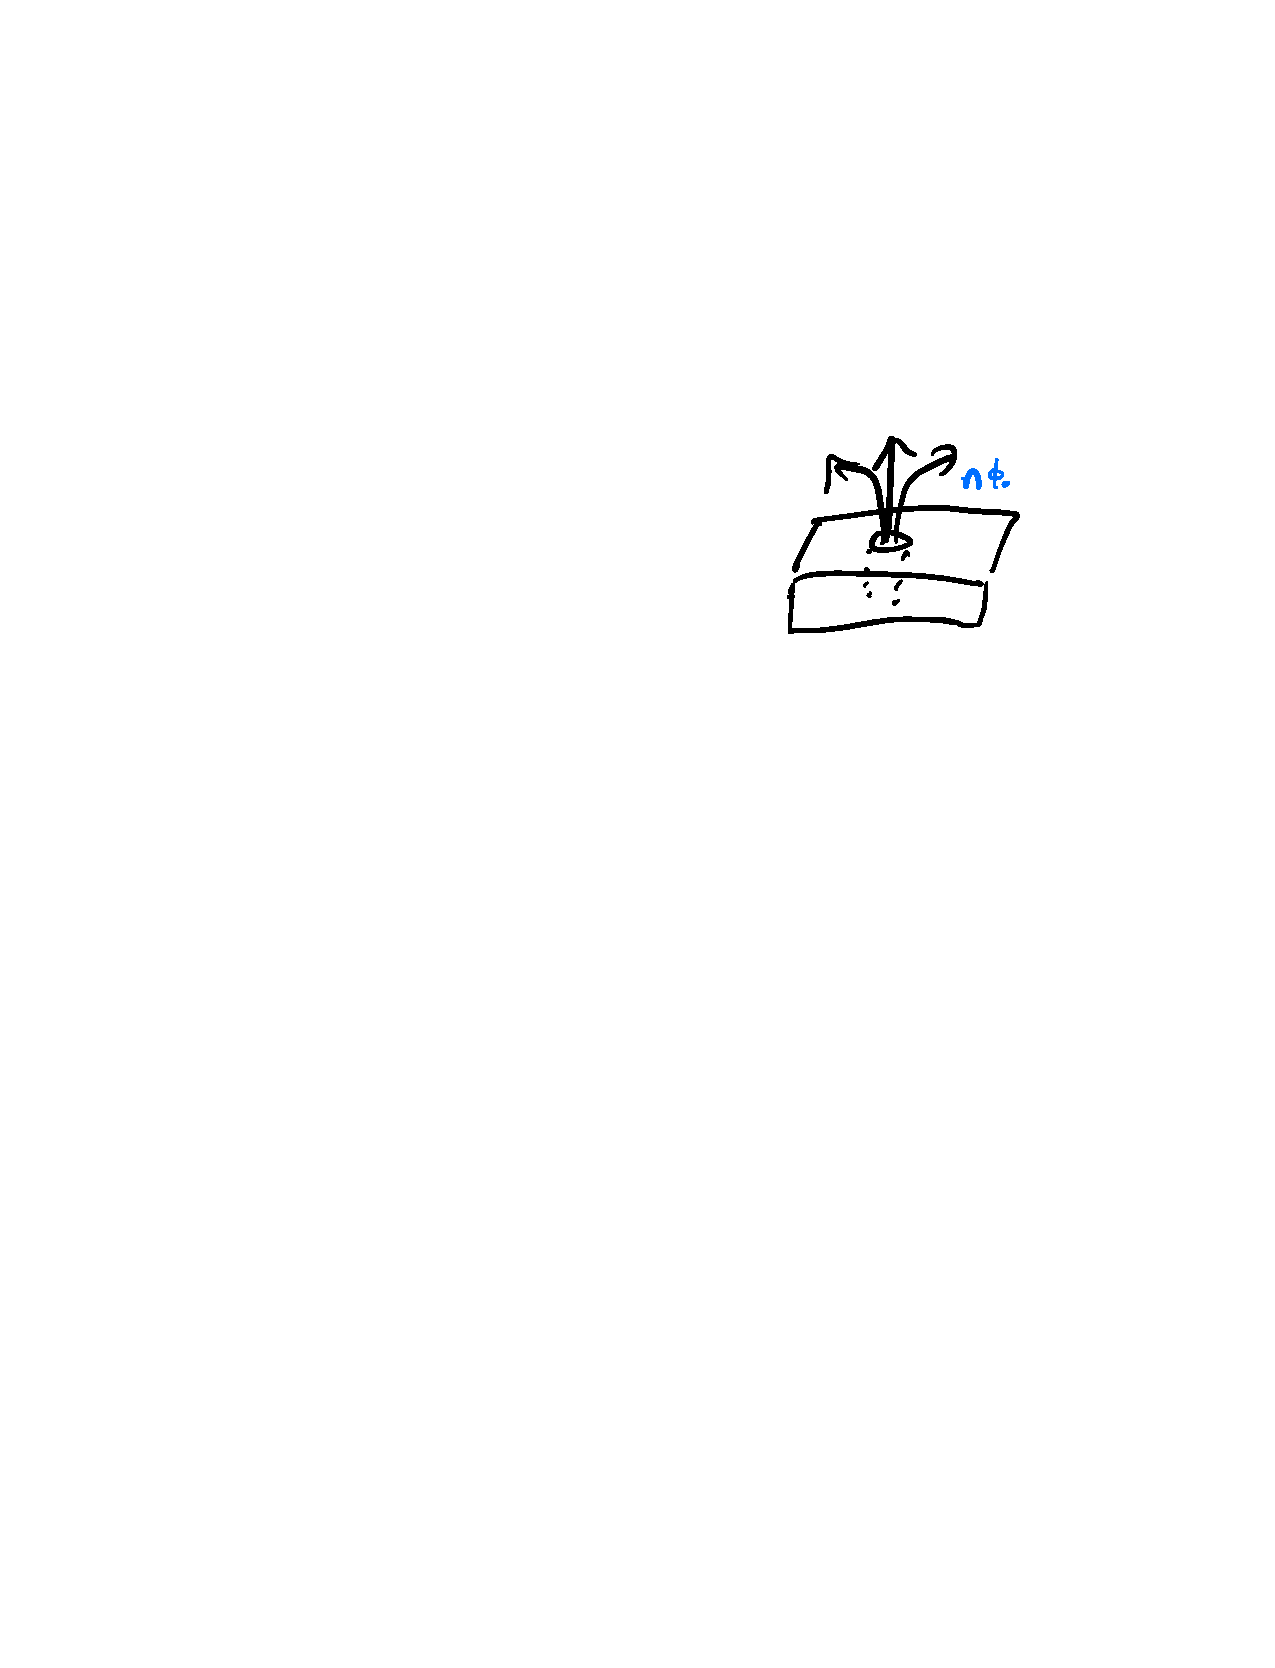
\includegraphics[scale=0.8]{Images/fig-quantizedflux.pdf}
        \caption{If we open a hole in a superconductor, the magnetic flux is quantized with $\Phi = n\Phi_0$.}
        \label{fig-quantizedflux}
    \end{figure}
\end{itemize}

How do we understand this effect? Note the theoryof superconductivity was developed in 1956, so it took almost 50 years from the discovery of the phenomenon before we got an explantory theory.

Note in 2011 (the 100 year anniversary of SC) a book was published with many famous papers (both theory and experiment), entertainingly many theory papers which were absolutely wrong.

\subsection{Cooper Instability}
Cooper instability\footnote{An interesting sociological point - when Cooper came up with this, he was actually a graduate student. He got a Nobel prize a few years later, but unfortunately didn't come up with anything else notable after this (though the other two awardees did). } is where for arbitrarily weak attractive interactions, electrons in a Fermi sea are unstable to formation of pairs, or electron-electron bound states. These are what are known as Cooper pairs. Superconductivity can be thought of as the condensation of e-e pairs, which act as bosons. Unlike Helium atoms which are charge neutral, cooper pairs carry a charge and therefore can carry current. The first clue to this is the $2e$ (rather than $e$) appearing in the superconducting flux quantum.

To discuss this problem, we consider $T = 0$ and consider the filled Fermi sphere.

Cooper considered two electrons that are slightly above the Fermi sphere, and considered the Hamiltonian of these two electrons:
\begin{equation}
    H = \frac{\v{p}_1^2}{2m} + \frac{\v{p}_2^2}{2m} + V(\v{r}_1 - \v{r}_2)
\end{equation}
we assume that the total momentum of the two is zero, so $\v{k}_1 + \v{k}_2 = \v{0}$. Further we assume that the electrons are in the spin singlet state (total spin is 0).

\begin{figure}[htbp]
    \centering
    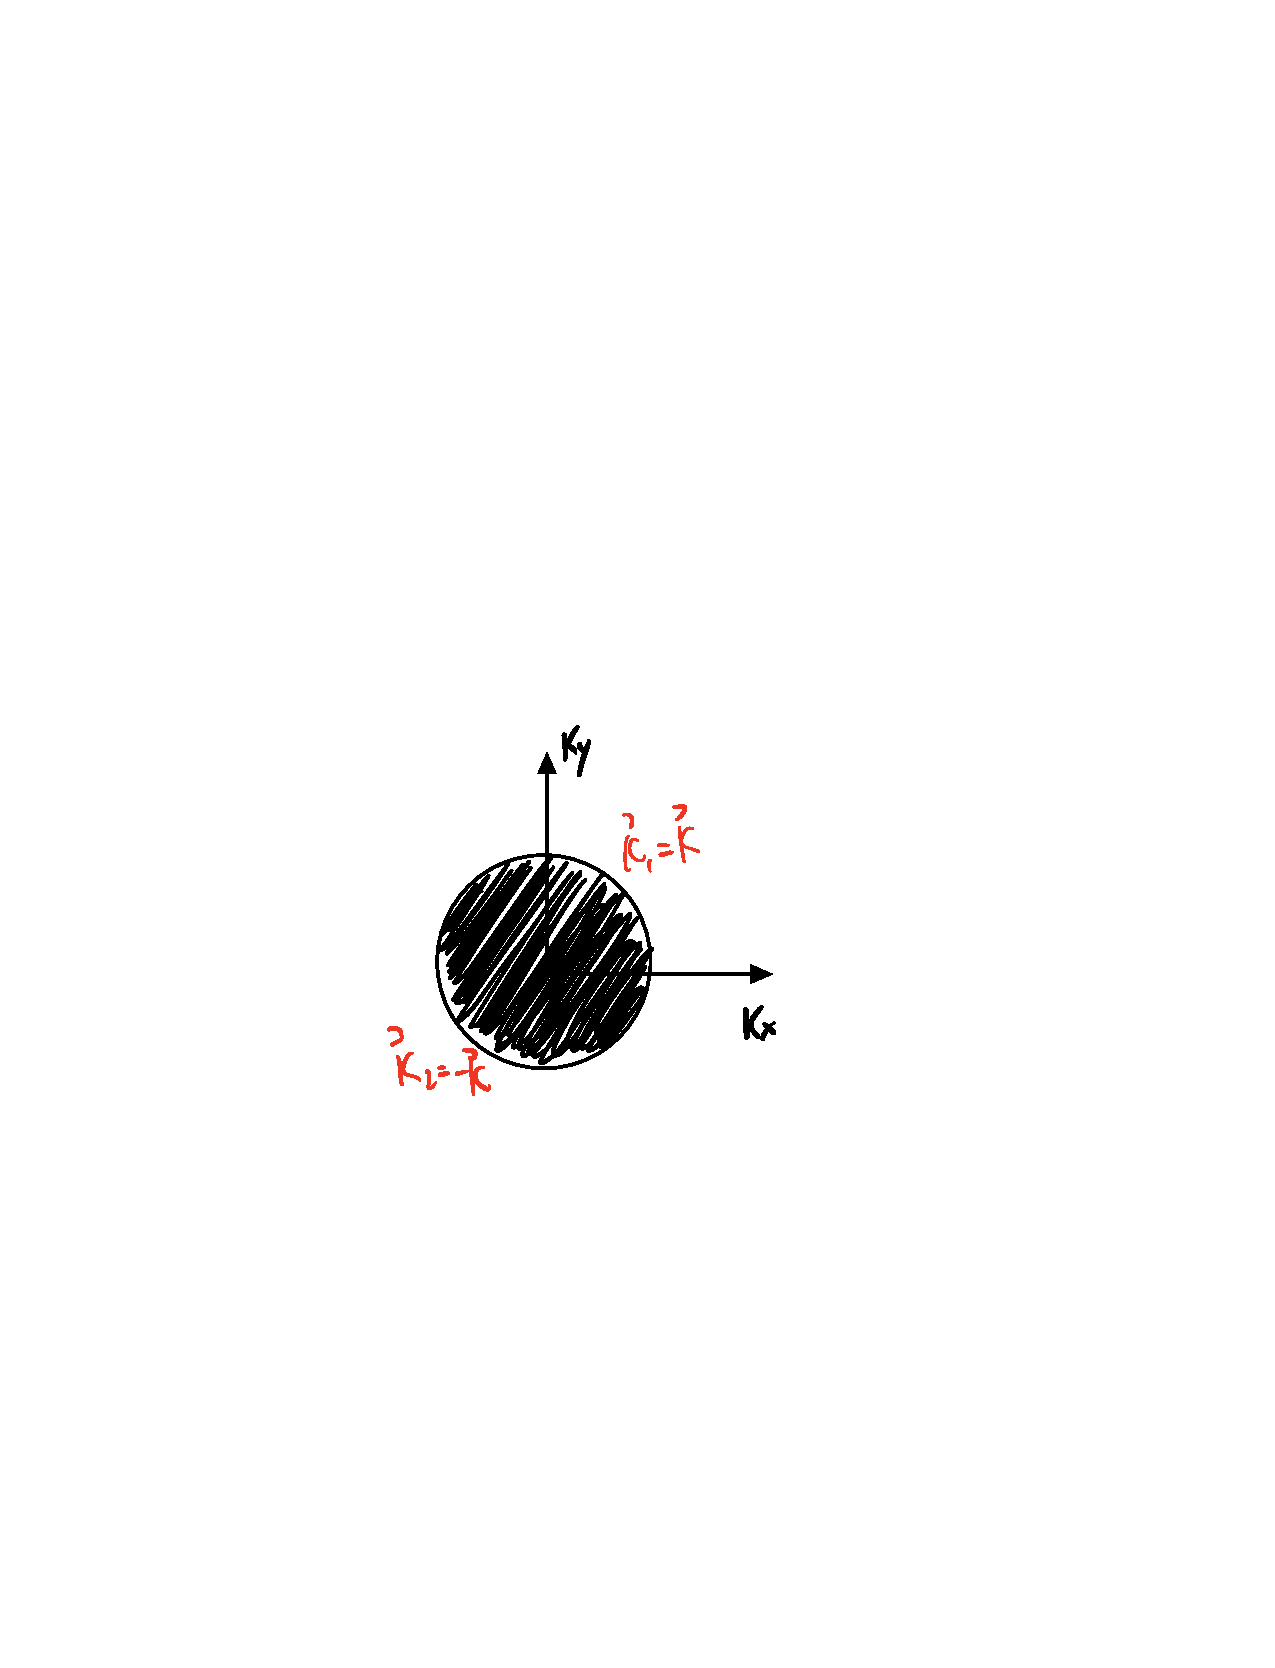
\includegraphics[scale=0.7]{Images/fig-cooperpairsetup.pdf}
    \caption{Setup of Cooper instability - We consider two electrons with total momentum zero, in a spin singlet state, sitting slightly above the Fermi sea.}
    \label{fig-cooperpairsetup}
\end{figure}

Under these assumptions, one is able to solve this problem. We make an ansatz:
\begin{equation}
    \psi(\v{r}_1, \v{r}_2) = \sum_{\abs{\v{k}} > k_F}g_{\v{k}} e^{i\v{k} \cdot \v{r}_1}e^{-i\v{k} \cdot \v{r}_2}\frac{\ket{\uparrow\downarrow} - \ket{\downarrow\uparrow}}{\sqrt{2}}
\end{equation}
Fermi statistics implies that $g_{\v{k}} = g_{-\v{k}}$. Because the spin part is already anti-symmetric, under interchange the $g$ part must be symmetric so under the interchange we have a net negative sign. From this, we can conclude that the wavefunction is only a function of the difference of the two coordinates:
\begin{align*}
    \psi(\v{r}_1 - \v{r}_2) = \sum_{\abs{\v{k}} > k_F}g_{\v{k}}\cos(\v{k} \cdot (\v{r}_1 - \v{r}_2)) \frac{\ket{\uparrow\downarrow} - \ket{\downarrow\uparrow}}{\sqrt{2}}
\end{align*}
Now, we look for $g_{\v{k}}$ by solving the Schrodinger equation with this Hamiltonian:
\begin{align*}
    H\psi_0 = E\psi_0
\end{align*}
What we get out is:
\begin{equation}
    (E - 2\e_{\v{k}})g_\v{k} = \sum_{\abs{\v{k}'} > k_F}V_{\v{k}\v{k}'}g_{\v{k}'}
\end{equation}
where $\e_{\v{k}} = \frac{\hbar^2\v{k}^2}{2m}$, and:
\begin{equation}
    V_{\v{k}, \v{k}'} = \frac{1}{\Omega}\int d^3r V(\v{r})e^{i(\v{k}' - \v{k}) \cdot \v{r}}
\end{equation}
now we make a Cooper ansatz for this interaction. If we take a generic interaction (such as that  we found from the el-ph interaction) we cannot solve this analytically. However, with the ansatz:
\begin{equation}
    V_{\v{k}\v{k}'} = \begin{cases}
        -V & \abs{\e_{\v{k}} - \e_F}, \quad \abs{\e_{\v{k}'} - \e_F } < \hbar \omega_c
        \\ 0 & \text{otherwise}
    \end{cases}
\end{equation}
With this ansatz:
\begin{align*}
    (E - 2\e_{\v{k}}) = -V\sum_{\v{k}'}'g_{\v{k}'}
\end{align*}
where the $'$ on the summation denotes the restriction of beign sufficiently close to the Fermi energy. From this we obtain:
\begin{align*}
    g_k = V\frac{\sum_{\v{k}'}' g_{\v{k}'}}{2\e_{\v{k}} - E}
\end{align*}
and so:
\begin{equation}
    \frac{1}{V} = \sum_{\v{k}}' \frac{1}{2\e_{\v{k}} - E}
\end{equation}
we now solve for the energy eigenvalue $E$ - we obtain this by going to the continuum approximation and replacing sum with integral:
\begin{equation}
    \frac{1}{V} = \int_{\e_F}^{\e_F + \hbar \omega_c} d\e N(\e)\frac{1}{2\e - E} = N(\e_F) \int_{\e_F}^{\e_F + \hbar \omega_c}d\e \frac{1}{2\e - E} = \frac{1}{2}N(\e_F)\ln\left(1 + \frac{2\hbar \omega_c}{2\e_F - E}\right)
\end{equation}
And we obtain the algebraic equation for $E$:
\begin{equation}
    1 + \frac{2\hbar \omega_c}{2\e_F - E} = e^{2/VN(\e_F)}
\end{equation}
If we make the weak coupling assumption of $VN(\e_F) \ll 1$, then the argument of the exponential becomes very large. Therefore we obtain the condition that $\e_F \approx E$. In this limit we can neglect the $+1$ on the LHS and solve for $E$ to be:
\begin{equation}
    E \approx 2\e_F - 2\hbar \omega_c e^{-\frac{2}{VN(\e_F)}}
\end{equation}
Normally, we would expect that $E > 2\e_F$ as the electrons should be above the Fermi surface (the Fermi sphere being full)! But with the attractive interaction, we find a state that has smaller energy than that - the attractive interaction lowers the energy. $E < 2\e_F$, meaning we have a bound state. Another point is that it exists at arbitrarily small $V > 0$. A final point - the expression is not analytic in $V$. This implies that Cooper instability is a non-perturbative phenomena. This is an important insight, and may explain why it took so long to formulate this theory - perturbative approaches to probe superconductivity are destined to fail, as $e^{-\frac{1}{V}}$ has no taylor expansion about $V = 0$- there is an essential singularity at $V = 0$.

Now the important thing to ask - what happens when we try to describe all the electrons? It is quite contrived to have a problem of a full Fermi sea and two extra electrons. However, it will nevertheless lead to the whole BCS theory of superconductivity we will discuss next lecture.

